\begin{figure}[h]
  \centering
  \begin{subfigure}[b]{0.48\textwidth}
    \centering    
    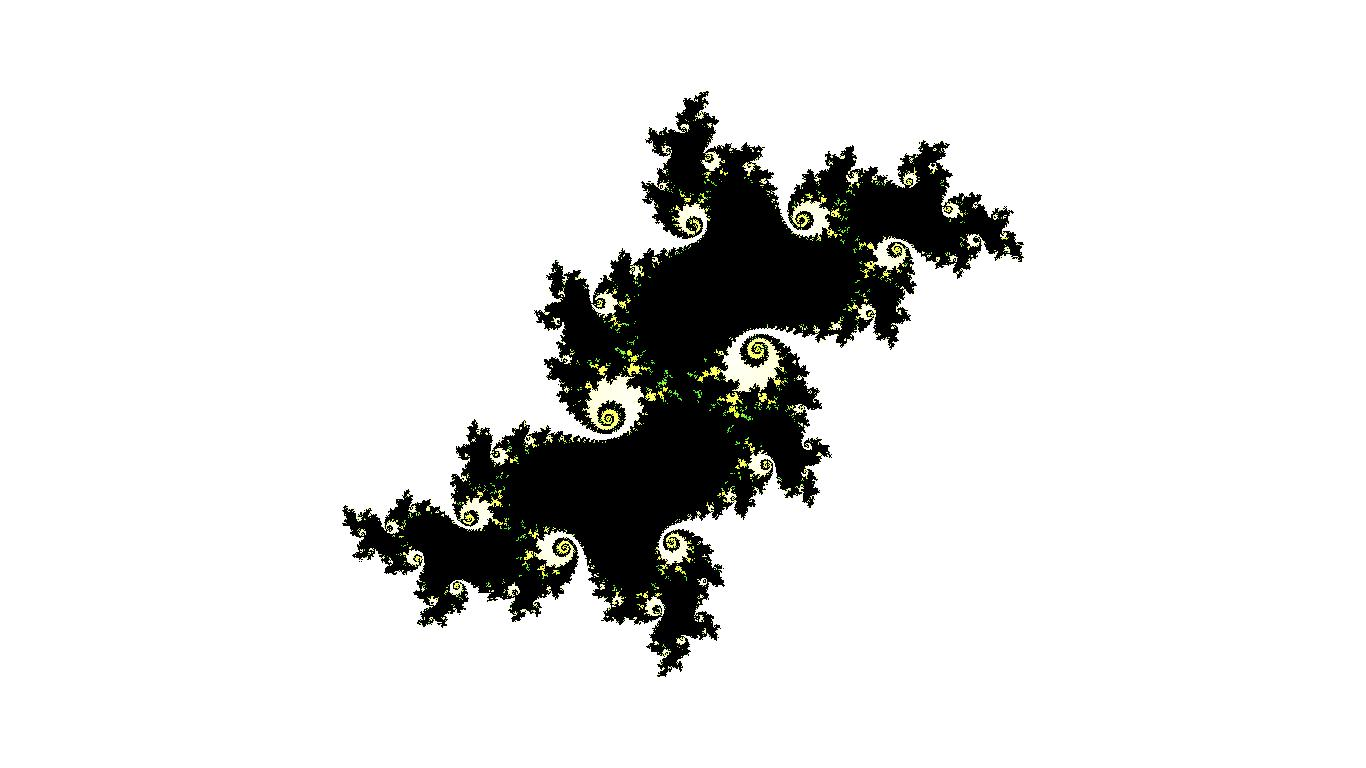
\includegraphics[width=\textwidth]{julia-con}
    \caption{
      \tiny The Julia Set for the complex \textit{c} value 
      \begin{math}
        (-0.1 + 0.649*i)
      \end{math}
    }
    \label{fig:juliaimgcon}
  \end{subfigure}
  ~ %spacer
  \begin{subfigure}[b]{0.48\textwidth}
    \centering
    
\includegraphics[width=\textwidth]{julia-ncon}
    \caption{
      \tiny The Julia Set for the complex \textit{c} value 
      \begin{math}
        (-0.75 + 0.03*i)
      \end{math}
    }
    \label{fig:juliaimgncon}
  \end{subfigure}
% full caption
  \caption{
    Two Julia Sets rendered using the program \textit{fraqtive}. 
    Figure \ref{fig:juliaimgcon} is a member of the Mandelbrot set. 
    Figure \ref{fig:juliaimgncon} is not.
  }
  \label{fig:juliaimgs}
\end{figure}
